\documentclass[11pt,a4paper]{article}
\usepackage[spanish]{babel}					% Utilizar español
\usepackage[utf8]{inputenc}					% Caracteres UTF-8
\usepackage{graphicx}						% Imagenes
\usepackage[hidelinks]{hyperref}			% Poner enlaces sin marcarlos en rojo
\usepackage{fancyhdr}						% Modificar encabezados y pies de pagina
\usepackage{float}							% Insertar figuras
\usepackage[textwidth=390pt]{geometry}		% Anchura de la pagina
\usepackage[nottoc]{tocbibind}				% Referencias (no incluir num pagina indice en Indice)
\usepackage{sectsty}						% Secciones sin enumeración
\usepackage{enumitem}						% Enumeraciones
\usepackage{mathtools}
\usepackage{amsmath}

% Configuracion de encabezados y pies de pagina
\pagestyle{fancy}
\lhead{Vladislav Nikolov Vasilev}
\rhead{Aprendizaje Automático}
\lfoot{Grado en Ingeniería Informática}
\cfoot{}
\rfoot{\thepage}
\renewcommand{\headrulewidth}{0.4pt}		% Linea cabeza de pagina
\renewcommand{\footrulewidth}{0.4pt}		% Linea pie de pagina

\begin{document}
\pagenumbering{gobble}

% Pagina de titulo
\begin{titlepage}

\begin{minipage}{\textwidth}

\centering


\includegraphics[scale=0.5]{img/ugr.png}\\

\textsc{\Large Aprendizaje Automático\\[0.2cm]}
\textsc{GRADO EN INGENIERÍA INFORMÁTICA}\\[1cm]

\noindent\rule[-1ex]{\textwidth}{1pt}\\[1.5ex]
\textsc{{\Huge MEMORIA PRÁCTICA 1\\}}
\noindent\rule[-1ex]{\textwidth}{2pt}\\[3.5ex]

\end{minipage}

\vspace{1.5cm}

\begin{minipage}{\textwidth}

\centering

\textbf{Autor}\\ {Vladislav Nikolov Vasilev}\\[2.5ex]
\textbf{Rama}\\ {Computación y Sistemas Inteligentes}\\[2.5ex]
\vspace{0.3cm}


\includegraphics[scale=0.3]{img/etsiit.jpeg}

\vspace{0.7cm}
\textsc{Escuela Técnica Superior de Ingenierías Informática y de Telecomunicación}\\
\vspace{1cm}
\textsc{Curso 2018-2019}
\end{minipage}
\end{titlepage}

\pagenumbering{arabic}
\tableofcontents
\thispagestyle{empty}				% No usar estilo en la pagina de indice

\newpage

\section{Ejercicio sobre la búsqueda iterativa de óptimos}

\subsection*{Apartado 1}
\noindent Implementar el algoritmo de gradiente descendente. \\

A continuación se muestra el código en Python implementado:

\begin{figure}[H]
\centering
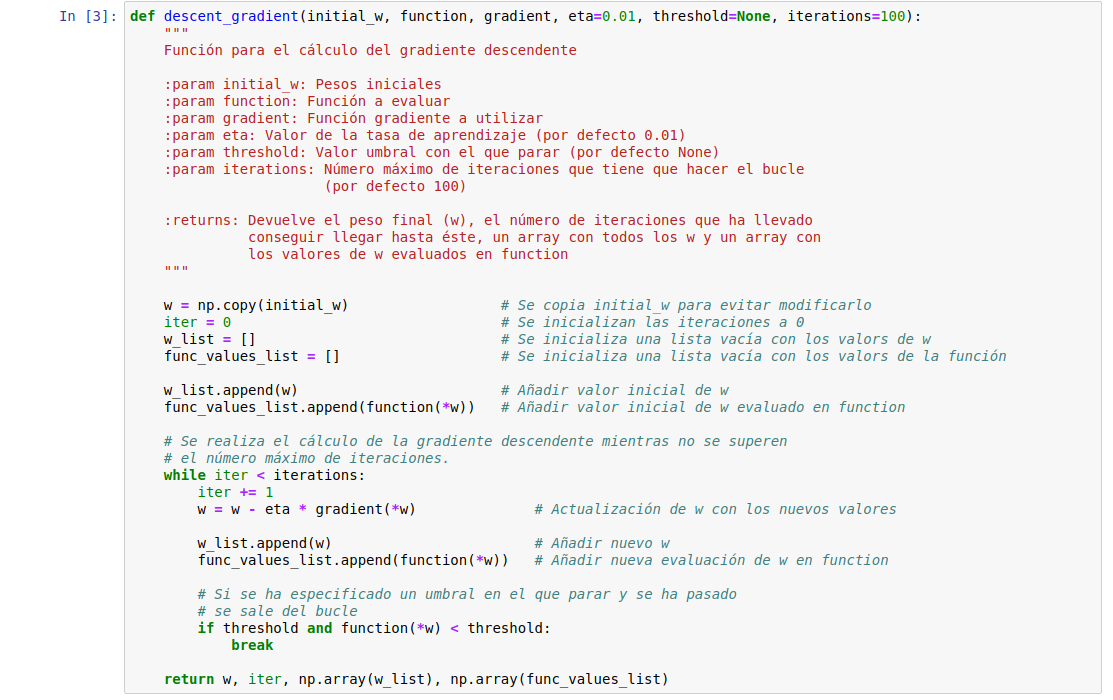
\includegraphics[scale=0.4]{img/descent_gradient_implementation.png}
\end{figure}


Se ha intentado que esta implementación sea lo más general posible para poder utilizarla en los ejercicios
posteriores, parametrizando la función que recibe (parámetro \textbf{function}), la cuál puede ser tanto
$f(x, y)$ como $E(u, v)$. Con este motivo, también se ha parametrizado el error con el que se quiere ajustar,
ya que en un caso no será necesario utilizar un error como criterio de parada (de ahí que su valor por defecto
sea \textbf{None}). Y, adicionalmente, se ha parametrizado el gradiente (parámetro \textbf{gradient}), para que
también se pueda especificar a la hora de la llamada cuál se usará. \\

\subsection*{Apartado 2}
\noindent Considerar la función $E(u, v) = (u^2 e^v - 2 v^2 e^{-u})^2$. Usar gradiente descendente para encontrar un
mínimo de esta funcón, comenzando desde el punto $(u, v) = (1, 1)$ y usanto una tasa de aprendizaje $\eta = 0.01$.

\begin{enumerate}[label=\alph*)]
	\item Calcular analíticamente y mostrar la expresión del gradiente de la función $E(u, v)$.
\end{enumerate}

Para calcular el gradiente, vamos a calcular antes $\frac{\partial E}{\partial u}$ y $\frac{\partial E}{\partial v}$.
Las derivadas, al aplicar la regla de la cadena, quedarían de la siguiente forma:

\begin{equation}
\begin{split}
\frac{\partial E}{\partial u}&= \frac{\partial}{\partial u} \Big( (u^2 e^v - 2 v^2 e^{-u})^2 \Big) = 2(u^2 e^v - 2 v^2 e^{-u})
\frac{\partial (u^2 e^v - 2 v^2 e^{-u})}{\partial u} = \\
 &=  2(u^2 e^v - 2 v^2 e^{-u})(2ue^v + 2 v^2 e^{-u})
\end{split}
\end{equation}

\begin{equation}
\begin{split}
\frac{\partial E}{\partial v}&= \frac{\partial}{\partial v} \Big( (u^2 e^v - 2 v^2 e^{-u})^2 \Big) = 2(u^2 e^v - 2 v^2 e^{-u})
\frac{\partial (u^2 e^v - 2 v^2 e^{-u})}{\partial v} = \\
 &=  2(u^2 e^v - 2 v^2 e^{-u})(u^2 e^v -4 v e^{-u})
\end{split}
\end{equation}

Con esto, tenemos que la expresión del gradiente es la siguiente:

\begin{equation}
\nabla E =
\left[ {
\begin{array}{c}
	\frac{\partial E}{\partial u} \\
	\\
	\frac{\partial E}{\partial v}
\end{array}
} \right]
\end{equation}

\begin{equation}
\nabla E =
\left[ {
\begin{array}{c}
	2(u^2 e^v - 2 v^2 e^{-u})(2ue^v + 2 v^2 e^{-u}) \\
	\\
	2(u^2 e^v - 2 v^2 e^{-u})(u^2 e^v -4 v e^{-u})
\end{array}
} \right]
\end{equation}

\begin{enumerate}[resume, label=\alph*)]
	\item ¿Cuántas iteraciones tarda el algoritmo en obtener por primera vez un valor de $E(u, v)$ inferior a $10^{-14}$?
	(Usar flotantes de 64 bits)
\end{enumerate}

El algoritmo tarda 33 iteraciones en encontrar el valor.

\begin{enumerate}[resume, label=\alph*)]
	\item ¿En qué coordenadas $(u, v)$ se alcanzó por primera vez un valor igual o menor a $10^{-14}$ en el apartado anterior?
\end{enumerate}

Las coordenadas donde se alcanzó un valor inferior a $10^{-14}$ son $(0.619, 0.968)$ (redondeadas a 3 cifras decimales).

\subsection*{Apartado 3}
\noindent Considerar ahora la función $f(x, y) = x^2 + 2y^2 + 2\sin(2 \pi x)\sin(2 \pi y)$.

\begin{enumerate}[label=\alph*)]
	\item Usar gradiente descendente para minimizar esta función. Usar como punto inicial $(x_0 = 0.1, y_0 = 0.1)$,
	tasa de aprendizaje $\eta = 0.01$ y un máximo de 50 iteraciones. Repetir el experimento pero usando $\eta = 0.1$,
	comentar las diferencias y su dependencia de $\eta$.
\end{enumerate}

\begin{enumerate}[resume, label=\alph*)]
	\item Obtener el valor mínimo y los valores de las variables $(x, y)$ en donde se alcanzan cuando el punto de inicio
	se fija: $(0.1, 0.1), (1, 1), (-0.5, -0.5), (-1, -1)$. Generar una tabla con los valores obtenidos.
\end{enumerate}

\subsection*{Apartado 4}
\noindent ¿Cuál sería su conclusión sobre la verdadera dificultad de encontrar el máximo global de una función arbitraria?

\section{Ejercicio sobre Regresión Lineal}

\section{Bonus}

\newpage

\begin{thebibliography}{5}

\bibitem{nombre-referencia}
Texto referencia
\\\url{https://url.referencia.com}

\end{thebibliography}

\end{document}

